\documentclass{standalone}

\usepackage{graphicx}

\usepackage{tikz}

\usetikzlibrary{positioning}
\usetikzlibrary{arrows.meta}

\begin{document}

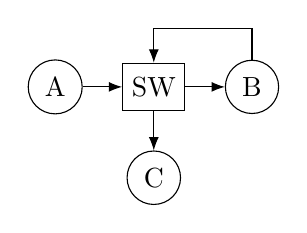
\begin{tikzpicture}[
	every node/.style={node distance=5mm},
	server/.style={rectangle, draw=black, fill=white, minimum size=0.6cm},
	switch/.style={rectangle, draw=black, fill=white},
	vm/.style={circle, draw=black, fill=white, node distance=5mm and 5mm},
]
	\node[vm]      	   	(V1)                        {A};
	\node[server]      	(S1)         [right=of V1]  {SW};
	\node[vm]			(V2)		 [right=of S1]	{B};
	\node[vm]			(V3)		 [below=of S1]  {C};

	\draw[-Latex] (V1.east) -- (S1.west);
	\draw[-Latex] (S1.east) -- (V2.west);
	\draw[-Latex] (V2.north) -| +(0,0.4) -| (S1.north);
	\draw[-Latex] (S1.south) -- (V3.north);
\end{tikzpicture}

\end{document}


